\chapter{Project execution}
This chapter contains the explanation of the groups working and development methods.
\section{Introduction}
We started this project with a lot of knowledge from previous projects. This knowledge lead us to the methods of working that we used throughout the project. The whole project was separated into phases and put on a time schedule. The time schedule is found in figure \ref{fig:TimeSched}.
\begin{figure}[H]
\centering
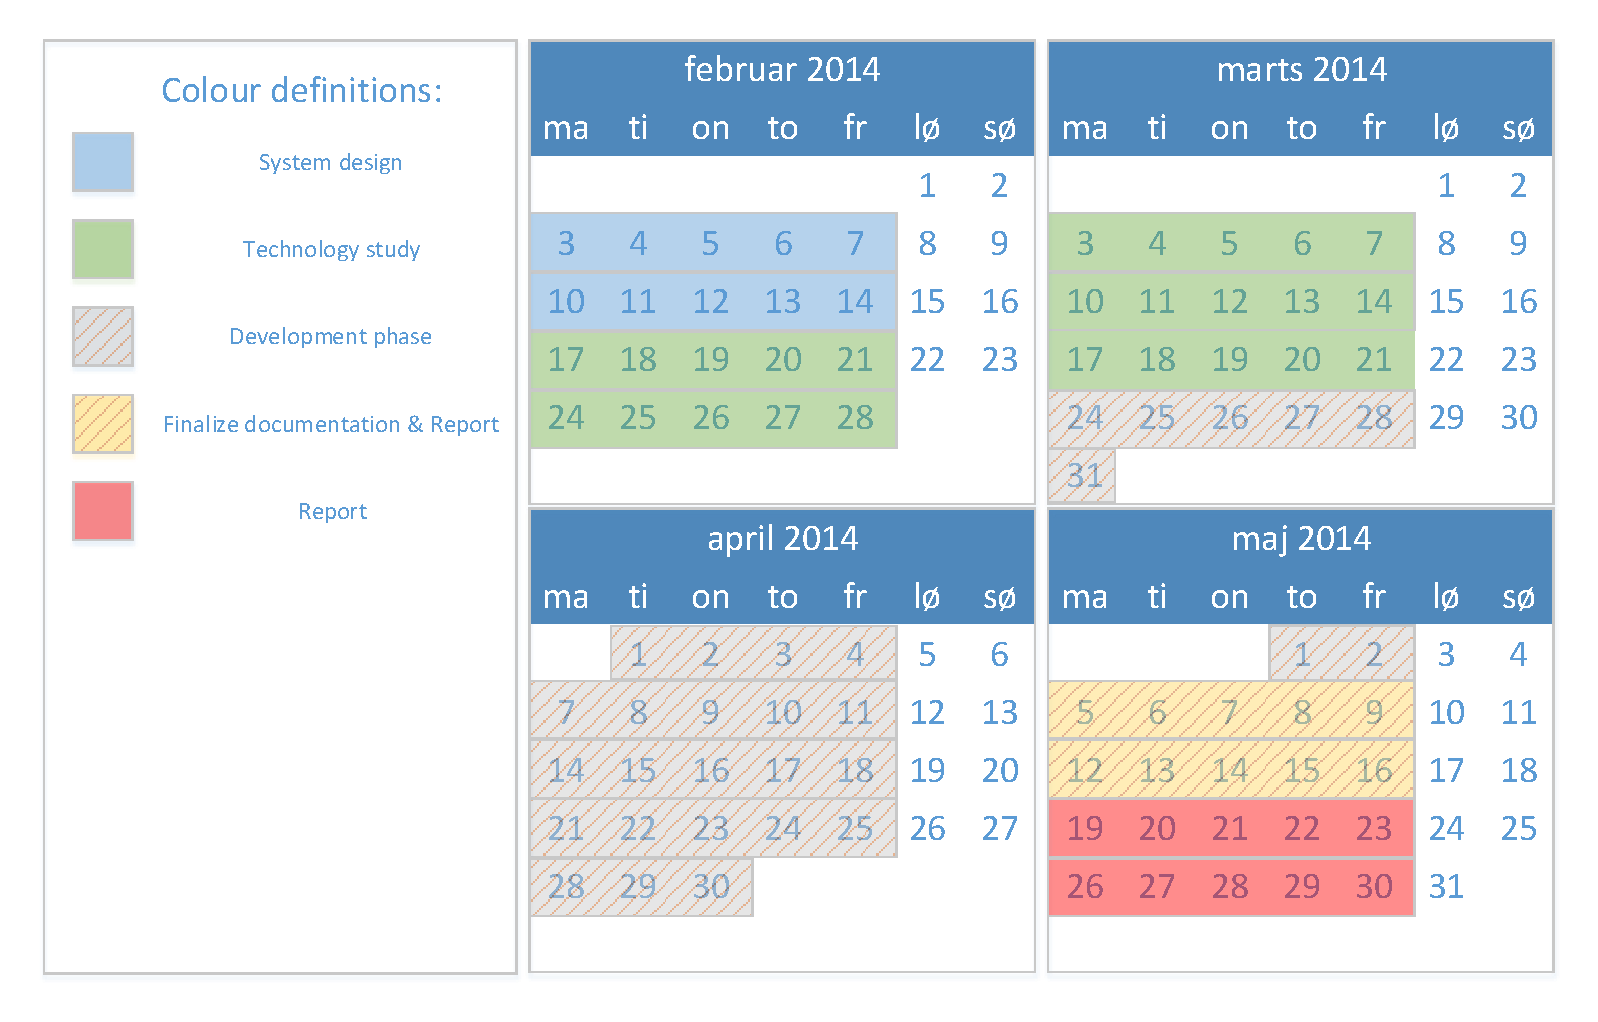
\includegraphics[width=0.8\textwidth]{billeder/Timeschedule_neat}
\caption{Time Schedule}
\label{fig:TimeSched}
\end{figure}
The phases we used are only describing the actual work in a very rough manner. These phases are:
\begin{itemize}
\item System design phase
\item Technology study phase
\item Development phase
\item Finalize documentation phase
\item Report phase
\label{it:phases}
\end{itemize}
Each phase gave way to one of more documents. The tree of the phases and documents are found in figure \ref{fig:doctree}.
\begin{figure}[H]
\centering
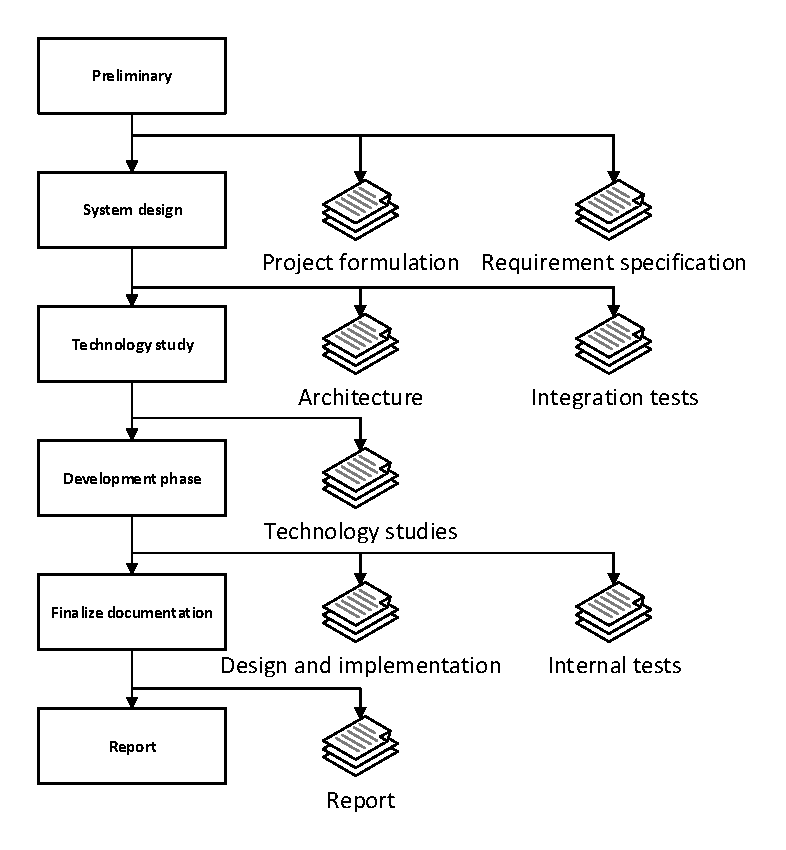
\includegraphics[width=0.6\textwidth]{billeder/DocumentTree}
\caption{Document Tree and Phases}
\label{fig:doctree}
\end{figure}

\section{Work method}
A project board was used to keep track of current and future tasks. Every day a board meeting was held with the following agenda:
\begin{itemize}
\item What did I accomplish yesterday?
\item What will I do today?
\subitem $\circ$ Todays "Must-Win" battles?
\item What obstacles are impeding my progress?
\subitem $\circ$ What will help me overcome this?
\end{itemize}
The tasks are equipped with an estimated time consumption. If a task stretches over 1 over more days, the time estimate is updated to reflect the future time consumption. An example of how the project board is structure is found in figure \ref{fig:prjboard}
\begin{figure}[H]
\centering
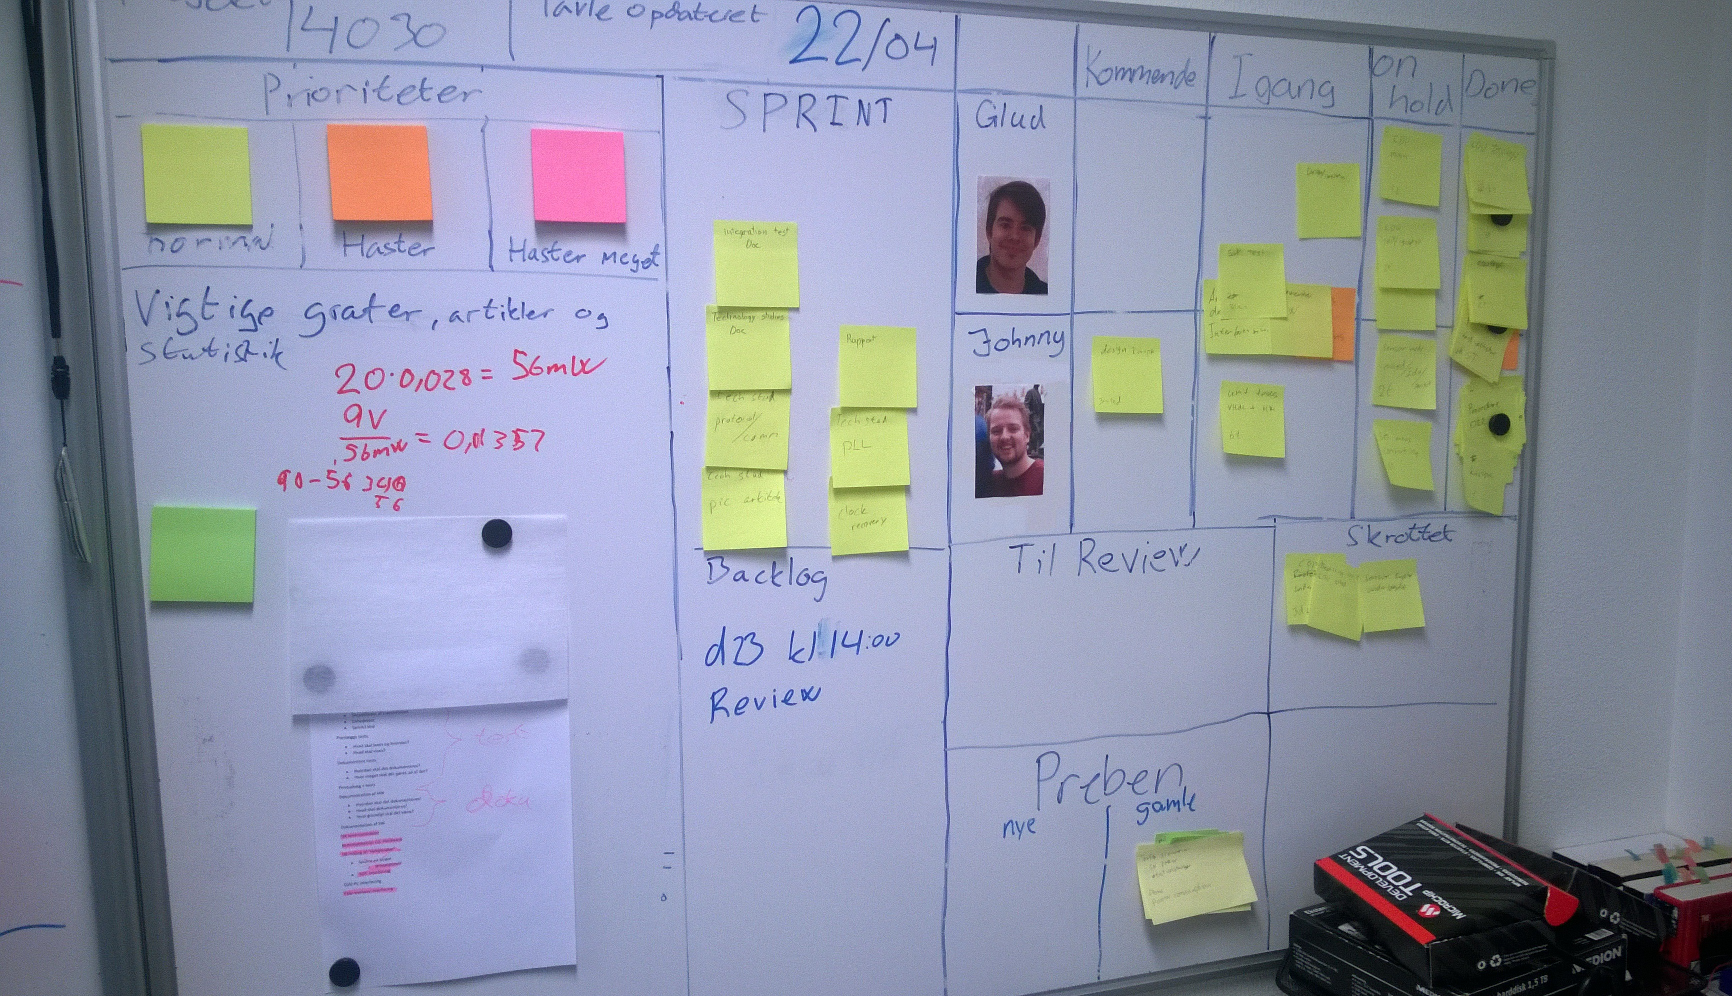
\includegraphics[width=0.8\textwidth]{billeder/board}
\caption{Project board}
\label{fig:prjboard}
\end{figure}

Every week a meeting with the project supervisor was held. The meeting was structured in the following way:
\begin{itemize}
\item Since last meeting
\item Present struggles/problems
\item Next weeks goals
\item Workrelated subjects
\item Closing remarks
\end{itemize}

Meetings

Review
